\chapter{Software Development Lifecycle (SDLC)}

Agile Methodology is a popular approach in SDLC that emphasizes flexibility, collaboration and customer satisfaction \cite{30} \cite{31}. The development process is broken down into sprints (small, incremental builds or iterations). Such an iterative process allows developers to focus on the most important features at any given moment, rather than strictly following a pre-defined plan. \\

Agile Methodology is guided by its four core values \cite{32}: 
\begin{enumerate}
    \item \textbf{Individuals and interactions} over processes and tools
    \item \textbf{Working software} over comprehensive documentation
    \item \textbf{Customer Collaboration} over contract negotiations
    \item \textbf{Responding to change} over following a plan 
\end{enumerate}


\begin{figure}
    \centering
    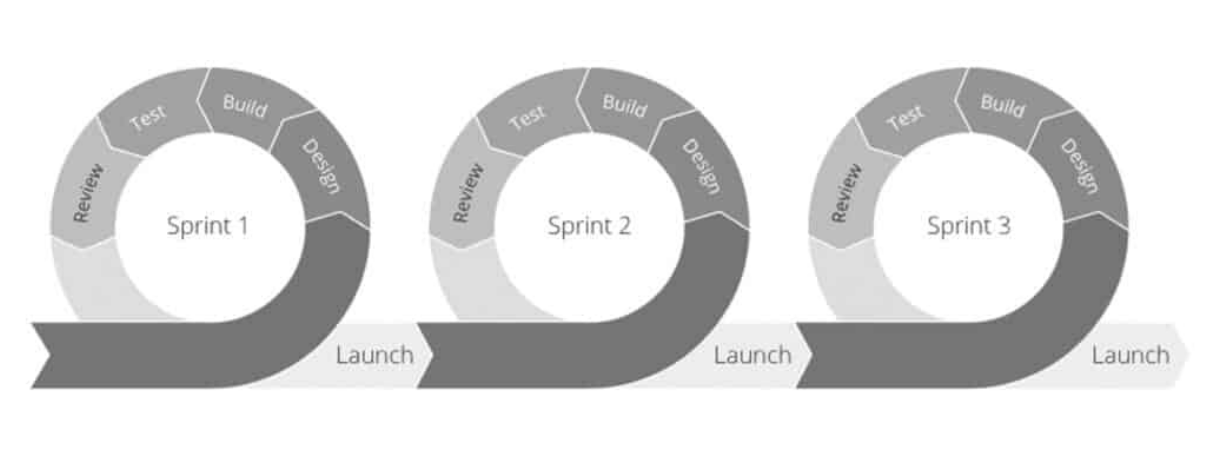
\includegraphics[width=1\linewidth]{images/sdlc.png}
    \caption{Anatomy of Agile Approach \cite{33}}
    \label{fig:sdlc}
\end{figure}



The adoption of this methodology especially in IoT and software development has been widespread for several reasons. 
\begin{itemize}
    \item \textbf{IoT:} Agile methodologies support multiple protocols and networks utilised for building IoT solutions. It enables closer cooperation between IoT hardware and software development teams, fostering higher transparency \cite{30}. This approach successfully addresses the complexity of connecting culture and technology in IoT implementation \cite{34}.
    \item \textbf{Software Development:} As per the 16th State of Agile Report by digital.ai, 78\% of the respondents report that they have implemented or are planning to implement Agile at scale. Agile’s emphasis on building working software quickly fostering cross-functional teams empowered to make decisions, and focusing on rapid iteration with continuous customer input are some of the reasons for its widespread adoption \cite{35}.  This approach not only follows better collaboration and incremental delivery but also provides early error detection and elimination of unnecessary work. 
\end{itemize}



\noindent Looking at the benefits of this approach, this project follows a similar approach. 
